% -*- coding: utf-8 -*-

\documentclass[a4paper,dvipdfmx]{jsarticle}
\usepackage{ascmac,alltt,txfonts,url}

\usepackage[dvipdfmx]{graphicx}
\usepackage{here}
\usepackage{fancyvrb}

\renewcommand{\ttdefault}{cmtt}
\renewcommand{\figurename}{図} 
\renewcommand{\tablename}{表} 
\DeclareMathAlphabet{\mathtt}{OT1}{cmtt}{m}{n}
\SetMathAlphabet{\mathtt}{bold}{OT1}{cmtt}{m}{n}
\setlength{\oddsidemargin}{0cm}
\setlength{\evensidemargin}{0cm}

\makeatletter

\newdimen\@mojihaba
\settowidth{\@mojihaba}{あ}

\def\tokushu#1{%
\def\tokushutitle{#1}%
\gdef\articleHeader{\hbox to\textwidth{\rule{3\@mojihaba}{1mm}%
\hbox{\small\bf\hskip1mm \tokushutitle}\leaderfill}}
}

\newdimen \JQ	\JQ .259817mm	%%%	\JQ/\Q = 10pt/9.62216pt
\newdimen \Q	\Q  .25mm	%%%	Quarter of 1mm

\def\JarticleHeader{\rule{\textwidth}{1mm}}%
\def\JarticleTitle{{\huge\bf\@title}}
\def\JarticleAuthor{\large\begin{tabular}[t]{@{}l}\@author\end{tabular}}
\newbox\@temptitlebox

\def\verse{\let\\=\@centercr 
 \list{}{\itemsep\z@ \itemindent -1.5em\listparindent \itemindent 
 \rightmargin\leftmargin\advance\leftmargin 1.5em}\item[]}
\let\endverse\endlist
\def\quotation{\list{}{\listparindent 1.5em
 \itemindent\listparindent
 \rightmargin\leftmargin \parsep 0pt plus 1pt}\item[]}
\let\endquotation=\endlist
\def\quote{\list{}{\rightmargin\leftmargin}\item[]}
\let\endquote=\endlist
\def\abstquotation{\list{}{\listparindent 1.5em
 \itemindent\listparindent
 \leftmargin 5mm
 \rightmargin\leftmargin \parsep 0pt plus 1pt}\item[]}
\let\endabstquotation=\endlist
\def\quote{\list{}{\rightmargin\leftmargin}\item[]}
\let\endquote=\endlist

\global\def\@maketitle{\newpage \null
\hbox{\vbox to193.5\Q{\baselineskip=10mm % 193.5\Q = 9*\baselineskip
\begin{flushleft}
\JarticleHeader
% following extra vskip together with baselineskip(10mm) will produce
% appropriate 10mm/6mm gap between the rule and title
% This assumes that title is typeset with 28Q(7mm) font, and baseline
% is set 1mm above the bottom of the font.
\setbox\@temptitlebox\hbox{JarticleTitle}\ifdim\wd\@temptitlebox>\textwidth\vskip2mm\else\vskip6mm\fi
\leftskip=5mm
\JarticleTitle
\vskip6mm % to leave 10mm gap between title and author
\JarticleAuthor
\end{flushleft}\vfil}}
%\JEabstInsert
  \begin{small}
    \begin{abstquotation}
      \Jabstcontent
    \end{abstquotation}
  \end{small}
}

\long\def\Jabstract#1{\global\long\def\Jabstcontent{\noindent\ignorespaces #1}}
\def\Jabstcontent{\relax}

\makeatother

\usepackage{fancyhdr}
\pagestyle{fancy}
\lhead{今どきのFPGA開発手法 - 高位合成の利用}
\rhead{}
\rhead{\thepage{}}
\cfoot{}
\renewcommand{\headrulewidth}{0.5pt}
\pagestyle{fancy}

\Jabstract{%
\\
FPGAを簡単に活用する手法として高位合成と呼ばれる開発手法に注目が集まっています.この章では,高位合成とは何か?について学びましょう.
}

\begin{document}

\title{今どきのFPGA開発手法 - 高位合成の利用}
\author{}
\date{2019年 8月22日~~第1.1版}
\maketitle

\section{高位合成とは?}\label{sec:overview}

FPGAを使うためには,長い間,VHDLあるいはVerilog HDLによるRTL設計が主流でした.しかし,HDLによるRTL設計は煩雑であり時間のかかる作業で簡単ではありません.そこで,最近では,高位合成という,HDLよりも高い水準での開発を可能する技術に注目が集まっています.特に,C/C++を利用したFPGA開発手法は,FPGAメーカーであるXilinxとIntelの両方から無償でツールが提供され,簡単にはじめられるようになりました.

この章では,実際に高位合成を使ってみる前に,高位合成とは何か,ということについて学んでおきましょう.

\subsection{FPGAとは - おさらい}
Field Programmable Gate Array(FPGA)は,プログラム可能なハードウェアデバイスであり,ユーザが自由にハードウェアロジックをその上に構築できます.そのため,ASIC開発のプロトタイプ環境としての利用に加え,アプリケーションに応じたユーザ独自の専用ハードウェア開発の環境としても利用されます.

FPGAを用いたアプリケーション開発では,プロセッサ上でソフトウェアとして実装する場合に比べ,並列性の活用による低消費電力で高い処理能力の実現が期待される.アーキテクチャを工夫し,データ並列性とパイプライン並列性を活用することで,プロセッサと比較して数十倍から数百倍以上の性能向上が得られます.

また,単に高速に演算処理を実現できるというだけではなく,FPGAはアプリケーションを構成する処理回路が入出力信号を直接操作することができるため,低レイテンシ,高スループットで物理デバイスにアクセスできる点に強みを持ちます.加えて,クロックレベルで決定的な処理を実装できることも,アプリケーションを専用ハードウェアとして実装するときの強みです.
現代的なプロセッサで動作するソフトウェアでは,キャッシュなどの実行支援ユニットの動作や,複数のプログラムのコンテクスト切り替えなどによって,実行タイミングや処理にかかる時間を正確に管理することが難しくなっています.
一方で,専用ハードウェアとしてアプリケーションを実装する場合には,クロック単位での信号の変化を自分で制御することができます.

\subsection{FPGAを使う...のは辛い}

FPGAの性能を効率良く活用するためには,一般に,VHDLやVerilogを用いたRTL設計が必要で,プロセッサ上で動作するソフトウェア開発に比べて,人的,時間的な開発コストが大きいのが問題でした.特に,アルゴリズムとして複雑な処理のRTL記述は繁雑で手間がかかり,時にはバグの温床となっています.
また,アプリケーションに合ったアーキテクチャで処理を実装することができれば高い演算性能を達成することができる一方で,そうでない場合には処理性能でプロセッサやASICを凌駕することは困難です.
そのため,FPGAで高性能処理を実現するためにアーキテクチャ上の試行錯誤をする必要があり,このこともまた,開発コストを大きくする要因です.

\subsection{高位合成の登場}

ソフトウェア開発のように,手軽にFPGA開発を行えるようにする取り組みとして,プログラムをハードウェアロジックに変換する技術が高位合成です.特に,C/C++で記述されたプログラムをハードウェアロジックに変換する高位合成処理系は,多数開発,販売されています.従来,実用に足るツールは高価だったのですが,2018年現在では,FPGAメーカーであるXilinxとIntelの両方からVivado HLSおよびIntel HLSコンパイラというツールが,無償で提供されるようになり導入のコストがぐっと小さくなりました.

自由にC/C++の記述能力を利用することはできないものの,C/C++のループや条件分岐などの制御構文や,処理を関数にまとめてそれを呼び出す処理分割といったメリットを享受することができます.信号処理をソフトウェアで実装した場合にありがちな多重のループ文に対してもパイプライン化やアンロールでハードウェアの特徴を活用できるようになったこと,ターゲット周波数によって実装方式の探索をさせられることなどから,場合によっては手でがんばってハードウェアを設計するよりも,よい回路を生成できることもあるようです.

\section{C/C++ベースのFPGA開発のながれ}
C/C++ベースのFPGAの開発,特にXilinxのVivado HLSを利用する流れを図\ref{fig:hls_dev_flow}に示します.要は,C/C++で記述したソースコードをVivado HLSによってVHDLまたはVerilog HDLに変換し,その変換後のコードをVivadoでFPGA用のビットストリームにする,というのが開発のおおまかな流れです.

 \begin{figure}[H]
  \begin{center}
   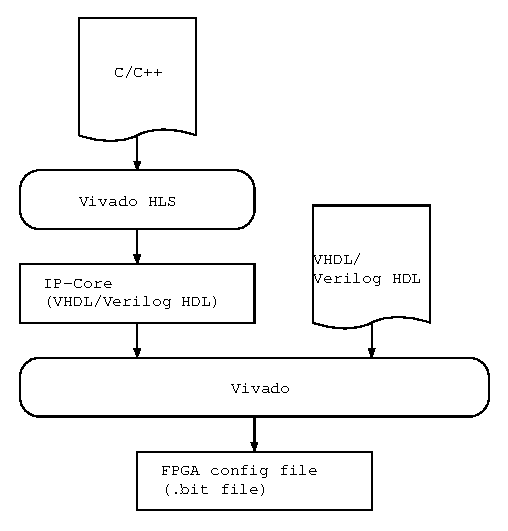
\includegraphics[width=.55\textwidth]{chapter07_figures/hls_dev_flow.eps}
  \end{center}
  \caption{Vivado HLSを使った開発フロー \label{fig:hls_dev_flow}}
 \end{figure}


C/C++ベースで作ったモジュールを設計に組み込むためには,ツールへの慣れは必要になりますが,特段難しいものではありません.次章以降,簡単なサンプルでステップを踏んでみていきましょう.

\end{document}
